\documentclass{ntuabeamer}
\usepackage[utf8]{inputenc}
\usepackage{amsmath,amssymb,graphicx,tikz}
\usepackage{appendixnumberbeamer}
\usetikzlibrary{arrows.meta,positioning,calc}
\graphicspath{{assets/generated/}}

\framesource{ho2020}{Ho, Jain, Abbeel. \emph{Denoising Diffusion Probabilistic Models}. NeurIPS, 2020.}
\framesource{song2021}{Song et al. \emph{Score-Based Generative Modeling through Stochastic Differential Equations}. ICLR, 2021.}

\title{Diffusion Models}
\author{}
\date{}
\definecolor{courseblue}{HTML}{3F7CAC}
\definecolor{courseorange}{HTML}{D97706}
\definecolor{coursegreen}{HTML}{27864A}
\definecolor{coursegray}{HTML}{667085}
\definecolor{coursepurple}{HTML}{7656A3}
\definecolor{coursered}{HTML}{B5473C}
\definecolor{courselightblue}{HTML}{DCE9F5}
\definecolor{courselightorange}{HTML}{F9E4C8}
\tikzset{flow/.style={-{Latex[length=3mm]},very thick,courseblue},
box/.style={draw,rounded corners,very thick,align=center,minimum width=1.6cm,minimum height=0.85cm}}

\begin{document}
\begin{frame}[plain]\makepresentationtitle\end{frame}

\section{Idea and Forward Process}
\sectiondivider{Part 1: Idea and Forward Process}

\begin{frame}{What a Generative Model Does}
  \[\mathbf x_0^{(1)},\ldots,\mathbf x_0^{(n)}\sim p_{\mathrm{data}}
    \quad\xrightarrow{\text{learn}}\quad
    \mathbf x_{\mathrm{new}}\sim p_\theta\approx p_{\mathrm{data}}\]
  \begin{itemize}
    \item \textbf{Generate:} draw new images, fields or simulation outputs.
    \item \textbf{Condition:} draw \(\mathbf x\sim p_\theta(\mathbf x\mid\mathbf c)\) for a label, prompt or boundary condition \(\mathbf c\).
    \item \textbf{Represent ambiguity:} draw several plausible outputs for the same request.
  \end{itemize}
\end{frame}

\begin{frame}{The Diffusion Idea: Destroy, Then Learn to Undo}
  \centering
  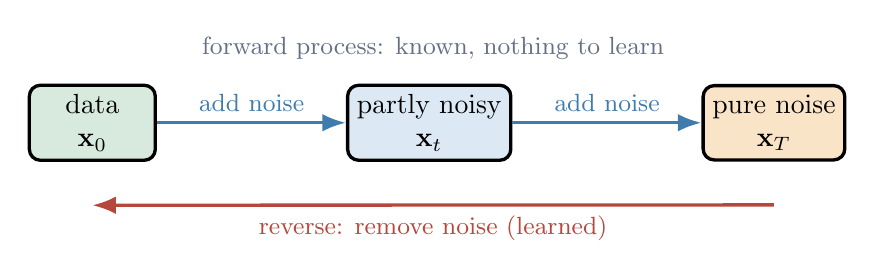
\begin{tikzpicture}[node distance=1.3cm]
    \node[box,fill=coursegreen!18] (data) {data\\\(\mathbf x_0\)};
    \node[box,fill=courselightblue,right=2.4cm of data] (mid) {partly noisy\\\(\mathbf x_t\)};
    \node[box,fill=courselightorange,right=2.4cm of mid] (noise) {pure noise\\\(\mathbf x_T\)};
    \draw[flow] (data) -- node[above,font=\small] {add noise} (mid);
    \draw[flow] (mid) -- node[above,font=\small] {add noise} (noise);
    \node[font=\small,coursegray] at ($(data)!0.5!(noise)+(0,0.95)$) {forward process: known, nothing to learn};
    \draw[-{Latex[length=3mm]},very thick,coursered] ([yshift=-0.55cm]noise.south) -- node[below,font=\small] {reverse: remove noise (learned)} ([yshift=-0.55cm]data.south);
  \end{tikzpicture}
  \vspace{0.3cm}
  \begin{itemize}
    \item Adding noise is easy and we know exactly how it works.
    \item Removing a \emph{little} noise is a small, learnable task.
    \item Generating = start from pure noise and remove noise step by step.
  \end{itemize}
  \textbf{So:} we turn one hard problem (create data) into many easy ones (clean up slightly).
\end{frame}

\begin{frame}{Forward Diffusion Gradually Destroys Structure}
  \centering
  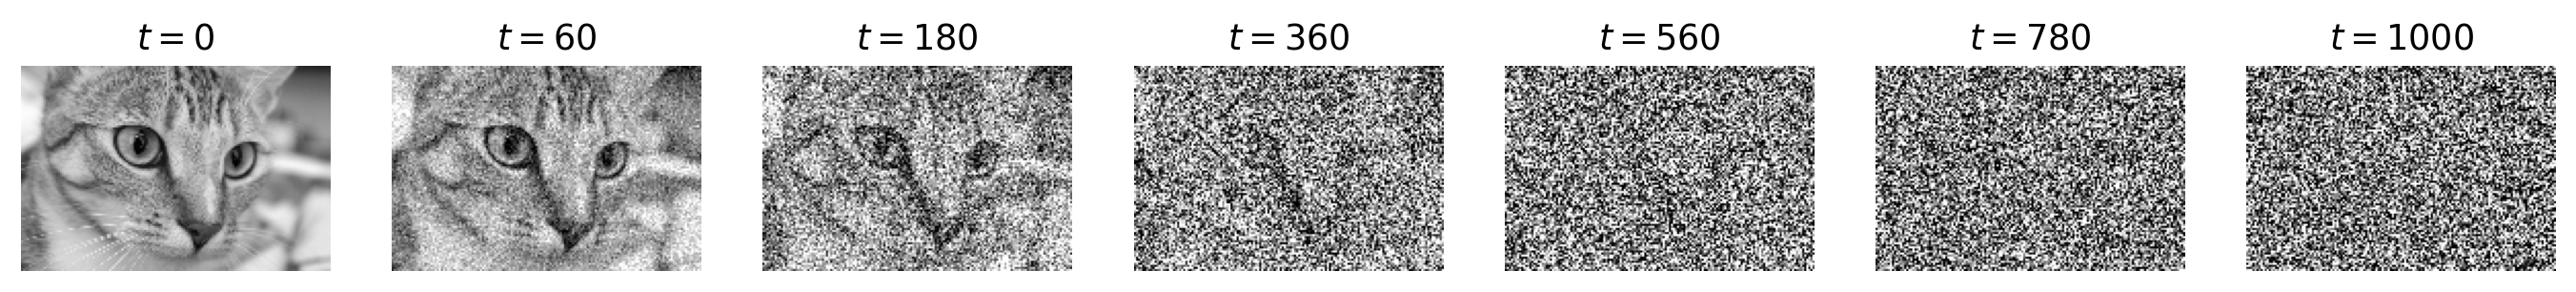
\includegraphics[width=0.95\textwidth,height=0.28\textheight,keepaspectratio]{diffusion_forward_chain_cat.png}
  \[\mathbf x_t=\sqrt{\alpha_t}\mathbf x_{t-1}+\sqrt{\beta_t}\boldsymbol\epsilon_t,\quad\alpha_t=1-\beta_t\]
  \[\mathbf x_t=\sqrt{\bar\alpha_t}\mathbf x_0+\sqrt{1-\bar\alpha_t}\boldsymbol\epsilon,\quad\bar\alpha_t=\prod_{s=1}^t\alpha_s\]
  \vspace{0.3cm}
  \begin{itemize}
    \item \textbf{Time convention in this deck:} \(t=0\) is clean data, \(t=T\) is pure noise
      (here \(T=1000\) steps). The flow-matching deck uses the opposite direction.
    \item Neighboring steps look alike, so undoing one step is a small task.
  \end{itemize}
  \textbf{So:} by \(t=T\) the picture is gone and only random noise remains.
\end{frame}

\begin{frame}{The Schedule: How Much Signal Is Left?}
  Write \(\alpha_t=1-\beta_t\) and let
  \(\bar\alpha_t=\alpha_1\alpha_2\cdots\alpha_t\) (a running product).
  \begin{itemize}
    \item \(\bar\alpha_t\) is the \textbf{fraction of the original signal power still left} at step \(t\).
    \item The list \(\beta_1,\ldots,\beta_T\) is the \emph{noise schedule}.
  \end{itemize}
  \begin{center}
  \begin{tabular}{r|ccccc}
    step \(t\) & 1 & 150 & 350 & 600 & 1000\\
    \hline
    \(\bar\alpha_t\) & 0.9999 & 0.79 & 0.29 & 0.026 & 0.00004
  \end{tabular}
  \end{center}
  (linear schedule, \(\beta_1=10^{-4}\) rising to \(\beta_T=0.02\)).

  \medskip
  \textbf{So:} \(\bar\alpha_t\) falls from 1 to almost 0: early states are mostly signal, late states mostly noise.
\end{frame}

\begin{frame}{A Toy Example in Two Dimensions}
  \centering
  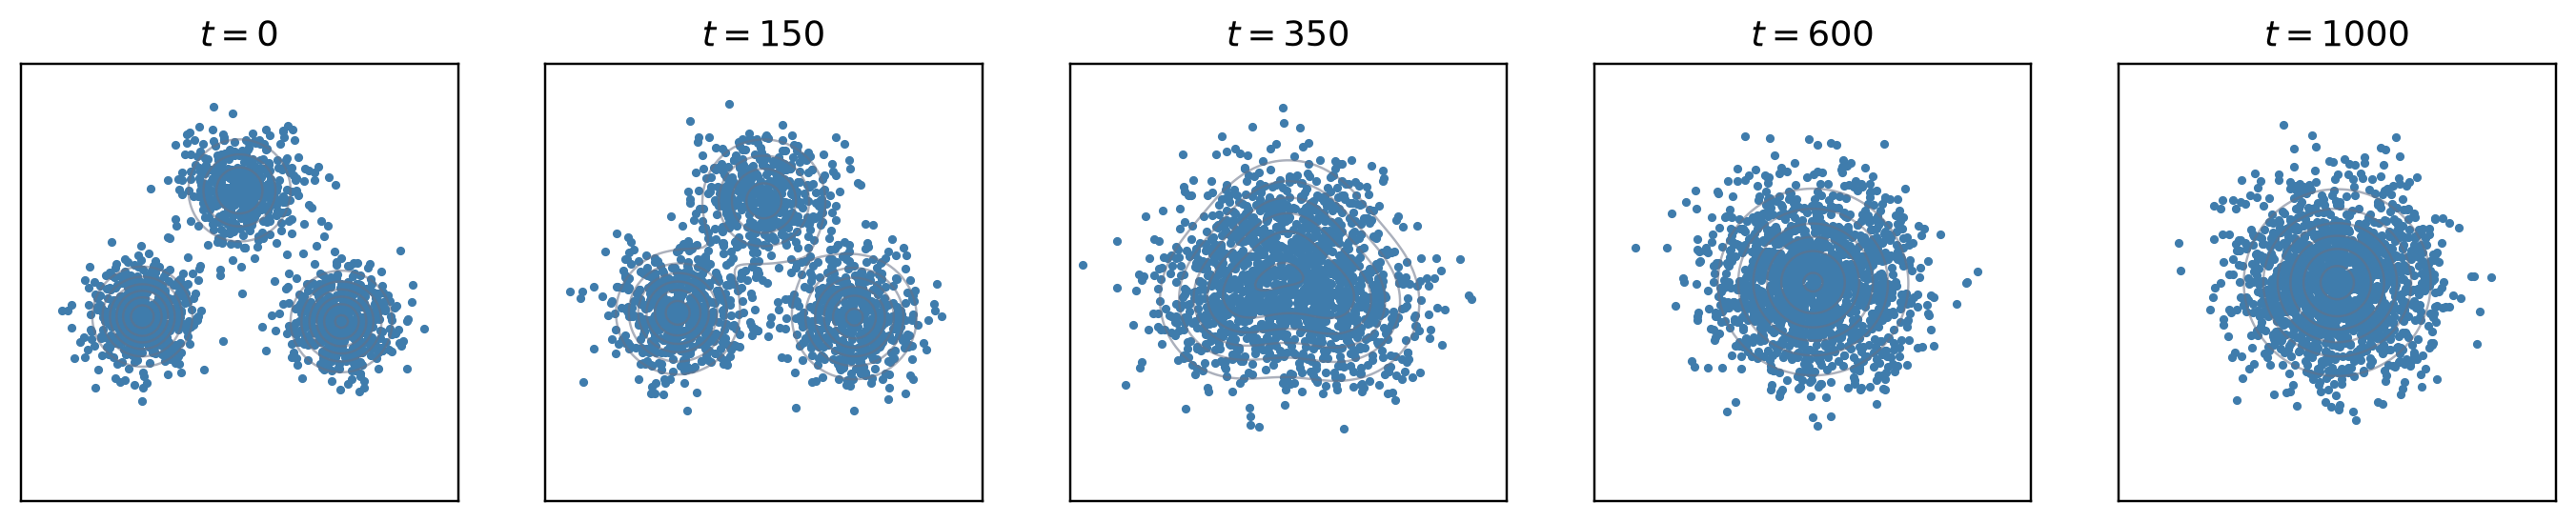
\includegraphics[width=0.98\textwidth]{diffusion_toy_forward.png}
  \vspace{0.2cm}
  \begin{itemize}
    \item Each dot is one sample \(\mathbf x_t\in\mathbb R^2\); the data are three clusters.
    \item Gray curves are level lines of the exact density of \(\mathbf x_t\) at that step.
  \end{itemize}
  \textbf{So:} noising melts three separate clusters into one round Gaussian blob.
\end{frame}

\section{Learning to Reverse}
\sectiondivider{Part 2: Learning to Reverse the Noise}

\begin{frame}{What Must Be Learned: Which Way Is ``Toward the Data''?}
  \[\boxed{\mathbf s_t(\mathbf x)=\nabla_{\mathbf x}\log p_t(\mathbf x)}\]
  \begin{itemize}
    \item \(p_t\): density of noisy samples at noise level \(t\).
    \item \textbf{Score:} local direction of increasing noisy-data density.
    \item Low noise: distinct clusters. High noise: blurred, ambiguous origins.
    \item The network needs \textbf{both} position \(\mathbf x_t\) and noise level \(t\).
  \end{itemize}
\end{frame}

\begin{frame}{The Score Points Toward Higher Density}
  \begin{columns}[c]
  \begin{column}{0.53\textwidth}
    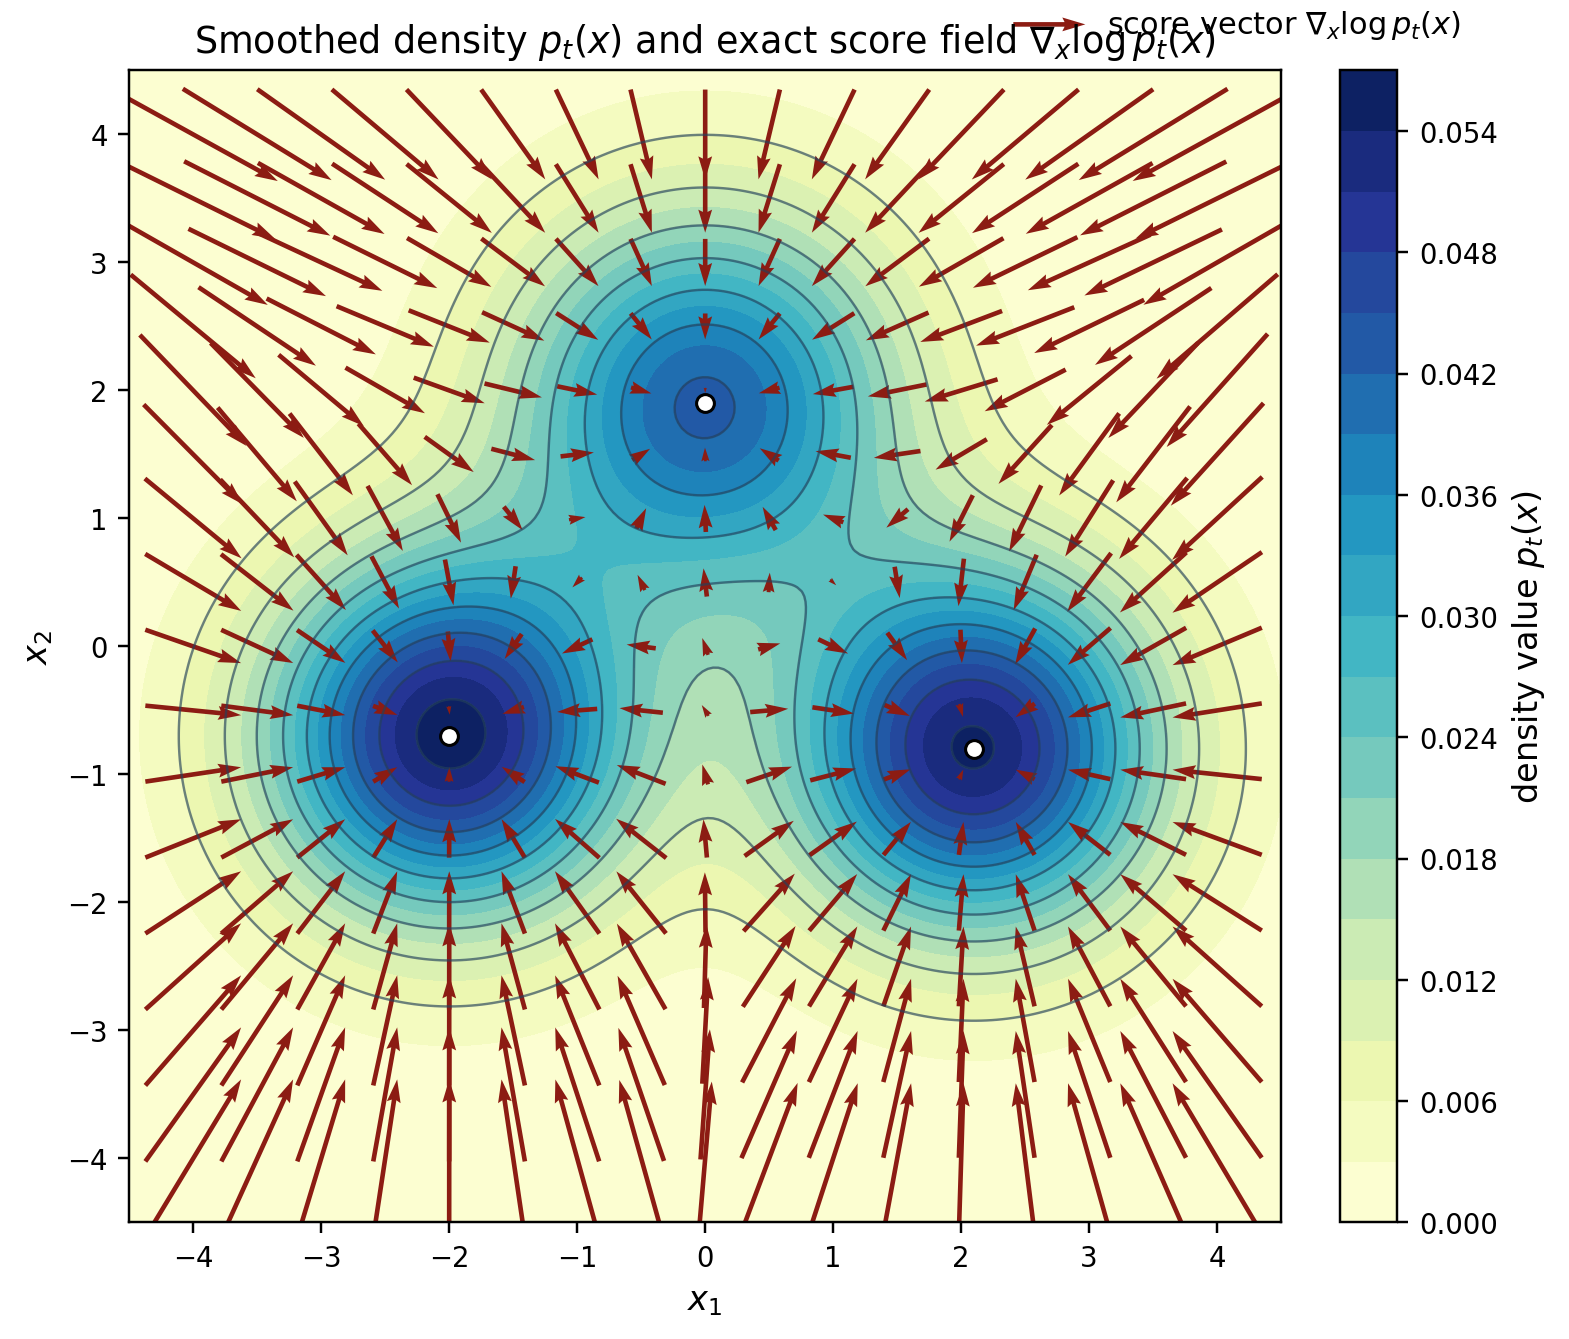
\includegraphics[width=\linewidth]{score_field_gaussian_mixture.png}
  \end{column}
  \begin{column}{0.47\textwidth}
    \[\mathbf s_t(\mathbf x)=\nabla_{\mathbf x}\log p_t(\mathbf x)\]
    Score arrows point toward higher noisy-data density.
    \[\mathbf s_t(\mathbf x)=-\frac{\mathbb E[\boldsymbol\epsilon\mid\mathbf x_t=\mathbf x]}{\sigma_t}\]
    \[\mathbf s_t(\mathbf x)\approx-\frac{\boldsymbol\epsilon_\theta(\mathbf x,t)}{\sigma_t}\]
    \(\sigma_t=\sqrt{1-\bar\alpha_t}\). Noise regression learns the score indirectly.
  \end{column}
  \end{columns}
\end{frame}

\begin{frame}{Training: One Step at a Time}
  \small
  \begin{center}
  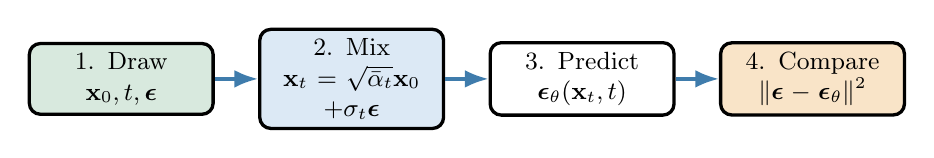
\begin{tikzpicture}[node distance=0.55cm,box/.append style={font=\small,minimum width=2.1cm,text width=2.1cm}]
    \node[box,fill=coursegreen!18] (draw) {1. Draw\\\(\mathbf x_0,t,\boldsymbol\epsilon\)};
    \node[box,right=of draw,fill=courselightblue] (mix) {2. Mix\\\(\mathbf x_t=\sqrt{\bar\alpha_t}\mathbf x_0\)\\\(+\sigma_t\boldsymbol\epsilon\)};
    \node[box,right=of mix] (net) {3. Predict\\\(\boldsymbol\epsilon_\theta(\mathbf x_t,t)\)};
    \node[box,right=of net,fill=courselightorange] (loss) {4. Compare\\\(\|\boldsymbol\epsilon-\boldsymbol\epsilon_\theta\|^2\)};
    \draw[flow] (draw)--(mix); \draw[flow] (mix)--(net); \draw[flow] (net)--(loss);
  \end{tikzpicture}
  \end{center}
  Draw \(t\) uniformly from \(1,\ldots,T\), and \(\boldsymbol\epsilon\sim\mathcal N(\mathbf0,\mathbf I)\). One jump supplies any noise level without simulating earlier steps.
  \[\boxed{L(\theta)=\mathbb E_{t,\mathbf x_0,\boldsymbol\epsilon}\|\boldsymbol\epsilon-\boldsymbol\epsilon_\theta(\mathbf x_t,t)\|^2}\]
  A time embedding tells the network the noise level; backpropagation updates its weights. Optional conditioning \(\mathbf c\) enters the network too.
\end{frame}

\begin{frame}{What the Network Actually Learns: The Average Noise}
  \[\boxed{\boldsymbol\epsilon_\star(\mathbf x_t,t)
    =\mathbb E[\boldsymbol\epsilon\mid\mathbf x_t,t]}\]
  \begin{itemize}
    \item Multiple clean examples can produce the same noisy observation.
    \item Squared error selects their \textbf{conditional mean noise}.
  \end{itemize}
  \textbf{Example:} equally likely \(x_0=\pm1\), observed \(x_t=0\):
  \[\epsilon=\mp\frac{\sqrt{\bar\alpha_t}}{\sigma_t}
    \quad\Longrightarrow\quad \mathbb E[\epsilon\mid x_t=0]=0.\]
  The individual noise is ambiguous; its conditional average gives the score.
\end{frame}

\section{Sampling and Control}
\sectiondivider{Part 3: Sampling and Control}

\begin{frame}{Sampling: Start From Noise and Remove It Step by Step}
  \begin{center}
  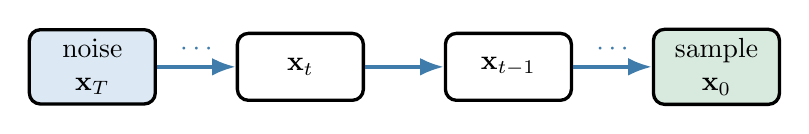
\begin{tikzpicture}[node distance=1.0cm]
    \node[box,fill=courselightblue] (a) {noise\\\(\mathbf x_T\)};
    \node[box,right=of a] (b) {\(\mathbf x_t\)};
    \node[box,right=of b] (c) {\(\mathbf x_{t-1}\)};
    \node[box,right=of c,fill=coursegreen!18] (d) {sample\\\(\mathbf x_0\)};
    \draw[flow] (a)--node[above] {\(\cdots\)} (b);
    \draw[flow] (b)--(c); \draw[flow] (c)--node[above] {\(\cdots\)} (d);
  \end{tikzpicture}
  \end{center}
  Start from \(\mathbf x_T\sim\mathcal N(\mathbf0,\mathbf I)\). For \(t=T,\ldots,1\):
  \[\boxed{\mathbf x_{t-1}=\frac1{\sqrt{\alpha_t}}\left(\mathbf x_t-\frac{\beta_t}{\sigma_t}\boldsymbol\epsilon_\theta(\mathbf x_t,t)\right)+\sqrt{v_t}\mathbf z}\]
  \(\mathbf z\sim\mathcal N(\mathbf0,\mathbf I)\) for \(t>1\); set \(\mathbf z=\mathbf0\) at the final step. The variance \(v_t\) is fixed or learned; the toy example uses the posterior variance \(\widetilde\beta_t\).
  Each step predicts noise, rescales the denoised state, and optionally adds fresh noise.
\end{frame}

\begin{frame}{A Real Sampler on the Toy Data}
  \centering
  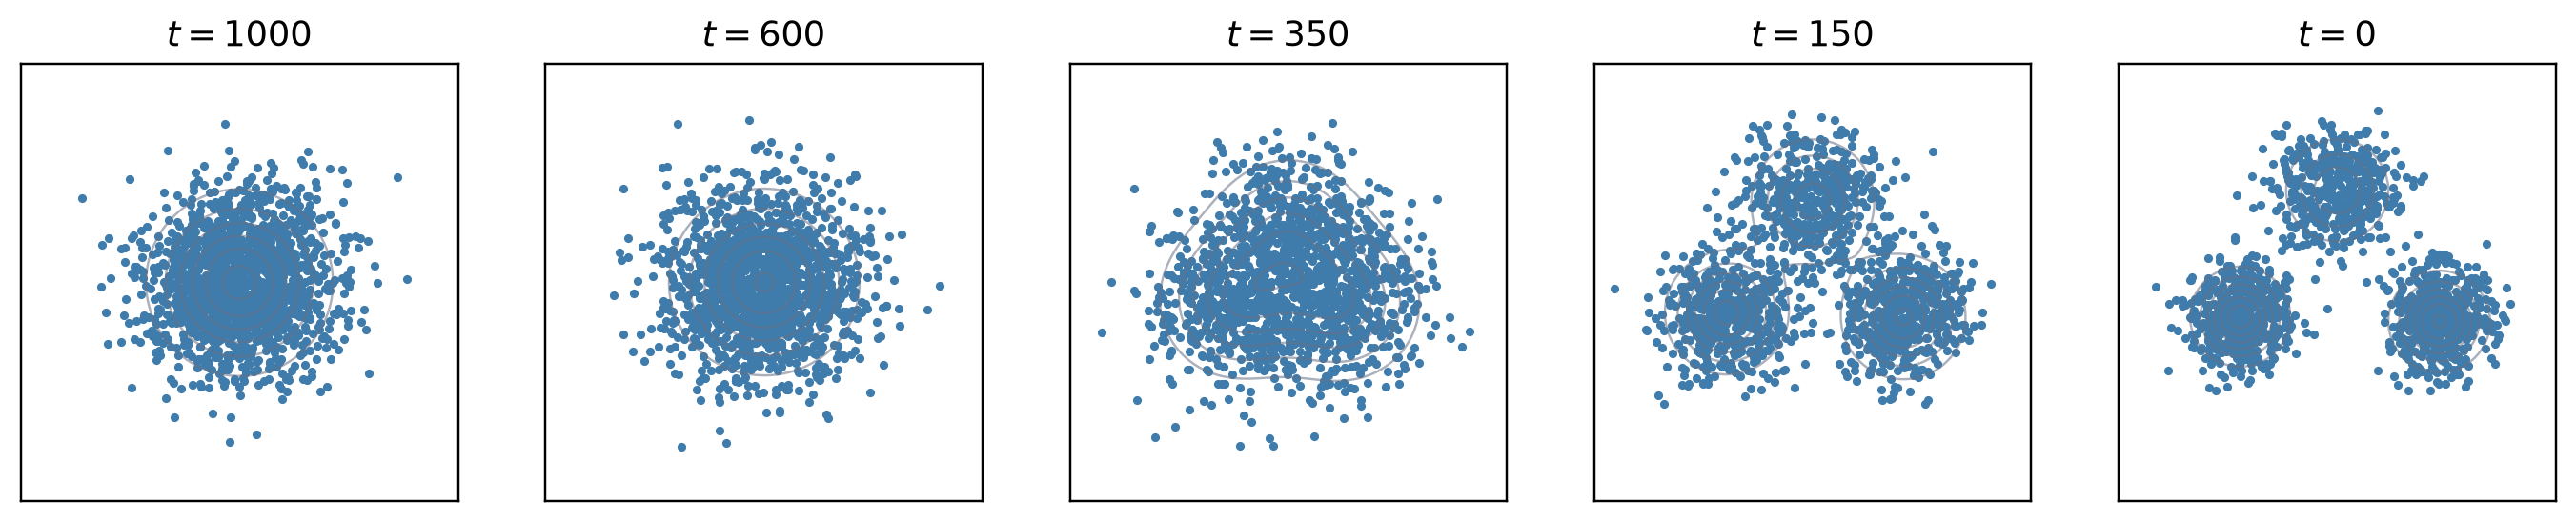
\includegraphics[width=0.98\textwidth]{diffusion_toy_reverse.png}
  \vspace{0.2cm}
  \begin{itemize}
    \item 1500 points start as pure noise at \(t=1000\) and are denoised down to \(t=0\).
    \item The data are never used: the exact score of this toy density plays the role of a trained network.
  \end{itemize}
  \textbf{So:} the three clusters emerge from noise alone, so the sampler really does generate.
\end{frame}

\begin{frame}{DDPM and DDIM Are Different Samplers}
  The same trained noise predictor supports different sampling rules.
  \begin{center}
  \begin{tabular}{p{2.0cm}p{3.6cm}p{3.6cm}}
    & DDPM & DDIM (deterministic)\\\hline
    Fresh noise & Yes, except final step & None (\(\eta_{\mathrm{DDIM}}=0\))\\
    Same start & Different outputs & Same output\\
    Time grid & Usually many steps & Often a reduced grid\\
    Tradeoff & Stochastic denoising & Fewer calls can reduce quality\\
  \end{tabular}
  \end{center}
  Report the sampler, time grid and network evaluations alongside sample quality. DDIM also has stochastic variants.
\end{frame}

\begin{frame}{Sampling Cost Is Counted in Network Evaluations}
  \begin{itemize}
    \item Every step costs at least one pass through the network.
    \item More steps usually mean smaller errors from the stepping itself, but slower generation.
    \item Guidance (next frames) can double the cost per step.
  \end{itemize}
  \[
    \text{sample quality}\;\approx\;\text{model error}+\text{stepping error}.
  \]
  \textbf{So:} a fair comparison states quality and the number of network evaluations together.
\end{frame}

\begin{frame}{Conditioning: Generating What You Ask For}
  Often we want a sample that matches information \(\mathbf c\): a class label, a text prompt, a boundary condition.
  \begin{itemize}
    \item Feed \(\mathbf c\) to the network as an extra input: \(\boldsymbol\epsilon_\theta(\mathbf x_t,t,\mathbf c)\).
    \item During training, drop \(\mathbf c\) at random (say 10\% of the time) so the same network also learns the unconditional guess.
  \end{itemize}
  \textbf{So:} one network now gives two guesses: with the condition and without it.
\end{frame}

\begin{frame}{Classifier-Free Guidance: Turning Up the Condition}
  Push the prediction further in the direction \(\mathbf c\) changes it:
  \[
    \boxed{\boldsymbol\epsilon_{\mathrm{guide}}
      =\boldsymbol\epsilon_{\mathrm{uncond}}
       +s\,(\boldsymbol\epsilon_{\mathrm{cond}}-\boldsymbol\epsilon_{\mathrm{uncond}})}
  \]
  \begin{itemize}
    \item \(s\) is the \textbf{guidance scale}, a number you choose at sampling time.
    \item \(s=1\): the ordinary conditional guess. \(s>1\): follow the condition more strongly.
    \item Reported effect: very large \(s\) lowers diversity and can create artifacts.
  \end{itemize}
  \textbf{So:} \(s\) is a dial between variety (low) and obeying the request (high).
\end{frame}

\section{Context and Evaluation}
\sectiondivider{Part 4: Context and Evaluation}

\begin{frame}{Continuous Time: Where the Flow-Matching Deck Takes Over}
  \begin{center}
  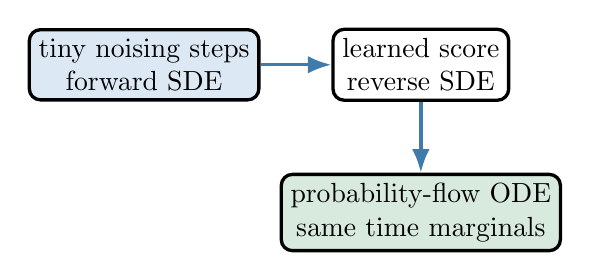
\begin{tikzpicture}[node distance=0.9cm]
    \node[box,fill=courselightblue] (f) {tiny noising steps\\forward SDE};
    \node[box,right=of f] (r) {learned score\\reverse SDE};
    \node[box,fill=coursegreen!18,below=of r] (o) {probability-flow ODE\\same time marginals};
    \draw[flow] (f)--(r); \draw[flow] (r)--(o);
  \end{tikzpicture}
  \end{center}
  \begin{itemize}
    \item SDE paths include random kicks; ODE paths are deterministic given the start.
    \item Matching marginals does not mean matching individual trajectories.
    \item Continuous-time formulas: flow-matching appendix.
  \end{itemize}
\end{frame}

\begin{frame}{Diffusion Applies Beyond Images}
  \begin{itemize}
    \item audio and time series,
    \item molecular and geometric structures,
    \item physical fields and ensembles of surrogate simulations,
    \item inpainting and inverse problems,
    \item uncertainty: many plausible outputs for one condition.
  \end{itemize}
  The noising process and the network must respect the data type; constraints (conservation,
  boundary values) usually need conditioning or projection, not only denoising.

  \medskip
  \textbf{So:} the recipe transfers, but the details must match the data.
\end{frame}

\begin{frame}{Evaluation Needs More Than Pretty Samples}
  \begin{itemize}
    \item Fidelity and diversity can conflict (see guidance).
    \item Check for memorization: are samples copies of training data?
    \item Conditional accuracy needs task-specific tests.
    \item Scientific samples should satisfy physical and statistical diagnostics.
    \item Report sampling cost: network evaluations and sampler settings.
  \end{itemize}
  \textbf{So:} judge a generator on quality, diversity, correctness and cost, not on one picture.
\end{frame}

\appendix
\sectiondivider{Appendix: optional depth}

\begin{frame}{Why the MSE Optimum Is a Conditional Average}
  For a random target \(\mathbf Y\) and input \(\mathbf X\),
  \[
    \arg\min_f\mathbb E\|\mathbf Y-f(\mathbf X)\|^2=\mathbb E[\mathbf Y\mid\mathbf X].
  \]
  Hence the ideal noise predictor is
  \[
    \boldsymbol\epsilon_\star(\mathbf x_t,t)=\mathbb E[\boldsymbol\epsilon\mid\mathbf x_t,t].
  \]
  The target noise is not uniquely recoverable from one noisy sample, so the minimizer is its conditional mean.
\end{frame}

\begin{frame}{Noise and Score Are Exactly Related}
  For fixed \(\mathbf x_0\),
  \[
    \nabla_{\mathbf x_t}\log q(\mathbf x_t\mid\mathbf x_0)
      =-\frac{\mathbf x_t-\sqrt{\bar\alpha_t}\mathbf x_0}{\sigma_t^2}
      =-\frac{\boldsymbol\epsilon}{\sigma_t}.
  \]
  Averaging at a fixed noisy state gives
  \[
    \boxed{\nabla_{\mathbf x_t}\log p_t(\mathbf x_t)
      =-\frac{\mathbb E[\boldsymbol\epsilon\mid\mathbf x_t,t]}{\sigma_t}}.
  \]
  Predicting the conditional mean noise therefore recovers the marginal score.
\end{frame}

\begin{frame}{The Exact Reverse Posterior Is Gaussian}
  If \(\mathbf x_0\) were known, conditioning the forward chain gives
  \[
    q(\mathbf x_{t-1}\mid\mathbf x_t,\mathbf x_0)
      =\mathcal N(\widetilde{\boldsymbol\mu}_t,\widetilde\beta_t\mathbf I),
  \]
  \[
    \widetilde{\boldsymbol\mu}_t
      =\frac{\sqrt{\bar\alpha_{t-1}}\beta_t}{1-\bar\alpha_t}\mathbf x_0
       +\frac{\sqrt{\alpha_t}(1-\bar\alpha_{t-1})}{1-\bar\alpha_t}\mathbf x_t,
    \qquad
    \widetilde\beta_t=\beta_t\frac{1-\bar\alpha_{t-1}}{1-\bar\alpha_t}.
  \]
  At generation time \(\mathbf x_0\) is unknown, so it is replaced by an estimate from the network.
\end{frame}

\begin{frame}{The DDPM Update Uses Predicted Noise}
  \small
  Substituting \(\mathbf x_0\) from the one-jump formula, with \(\boldsymbol\epsilon\) replaced by \(\boldsymbol\epsilon_\theta\), gives
  \[
    \boxed{\boldsymbol\mu_\theta(\mathbf x_t,t)
      =\frac1{\sqrt{\alpha_t}}\left(\mathbf x_t-\frac{\beta_t}{\sigma_t}\,\boldsymbol\epsilon_\theta(\mathbf x_t,t)\right)},
    \qquad
    p_\theta(\mathbf x_{t-1}\mid\mathbf x_t)=\mathcal N(\boldsymbol\mu_\theta,v_t\mathbf I).
  \]
  The variance \(v_t\) is fixed (for example \(\beta_t\) or \(\widetilde\beta_t\)) or learned.
  The toy sampler in the main text uses \(v_t=\widetilde\beta_t\).
\end{frame}

\begin{frame}{Reverse Updates When \(\mathbf x_0\) Is Known (an Oracle, Not a Sampler)}
  \centering
  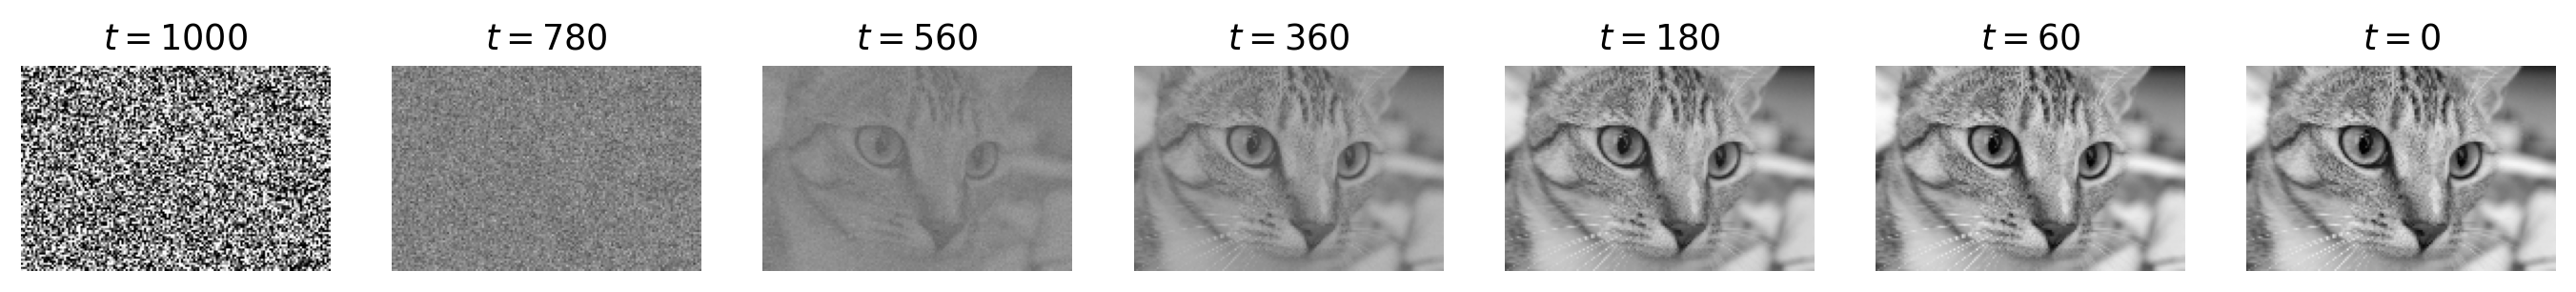
\includegraphics[width=0.95\textwidth]{diffusion_reverse_chain_cat_oracle.png}
  \vspace{0.3cm}
  \begin{itemize}
    \item Each step applies the exact posterior mean, which uses the true clean image \(\mathbf x_0\).
    \item This shows the geometry of the update only. It cannot generate new images, because \(\mathbf x_0\) is known.
    \item A real sampler replaces \(\mathbf x_0\) by the network's estimate (previous toy example).
  \end{itemize}
\end{frame}

\end{document}
